\documentclass[submit]{harvardml}

% FDV: Update front matter -- years, dates, references to book sections, etc.
\course{CS181-S22}
\assignment{Assignment \#5}
\duedate{11:59pm EST, April 8, 2021}

\newcommand{\attr}[1]{\textsf{#1}}
\usepackage[OT1]{fontenc}
\usepackage[colorlinks,citecolor=blue,urlcolor=blue]{hyperref}
\usepackage[pdftex]{graphicx}
\usepackage{subfig}
\usepackage{framed}
\usepackage{fullpage}
\usepackage{amsmath}
\usepackage{amssymb}
\usepackage{color}
\usepackage{todonotes}
\usepackage{listings}
\usepackage{common}
\usepackage{bm}
\usepackage{enumitem}
\usepackage{tikz}
\usetikzlibrary{positioning,shapes,arrows}
\usepackage{xifthen}
\usepackage{pythonhighlight}
\usepackage{soul}

\usepackage[mmddyyyy,hhmmss]{datetime}

\definecolor{verbgray}{gray}{0.9}

\lstnewenvironment{csv}{
  \lstset{backgroundcolor=\color{verbgray},
  frame=single,
  framerule=0pt,
  basicstyle=\ttfamily,
  columns=fullflexible}}{}

\begin{document}


\begin{center}
{\Large Homework 5: EM with Mixtures, PCA, and Graphical Models}\\
\end{center}

This homework assignment will have you work with EM for mixtures, PCA,
and graphical models. We encourage you to read sections 9.4 and 8.2.5 of the course textbook.

Please type your solutions after the corresponding problems using this
\LaTeX\ template, and start each problem on a new page.

Please submit the \textbf{writeup PDF to the Gradescope assignment `HW5'}. Remember to assign pages for each question.

Please submit your \textbf{\LaTeX\ file and code files to the Gradescope assignment `HW5 - Supplemental'}. 


\newpage
\begin{problem}[Expectation-Maximization for Gamma Mixture Models, 25pts]

In this problem we will explore expectation-maximization for a Categorical-Gamma Mixture model.

Let us suppose the following generative story for an observation $x$: first one of $K$ classes is randomly selected, and then the features $x$ are sampled according to this class. If $$z \sim \operatorname{Categorical}(\btheta)$$ indicates the selected class, then $x$ is sampled according to the class or ``component'' distribution corresponding to $z$. (Here, $\btheta$ is the mixing proportion over the $K$ components: $\sum_k \theta_k = 1$ and $ \theta_k > 0$). In this problem, we assume these component distributions are gamma distributions with shared shape parameter but different rate parameters: $$x | z \sim \operatorname{Gamma}(\alpha, \beta_k).$$

In an unsupervised setting, we are only given a set of observables as our training dataset: $\mathcal D = \{x_n\}_{n=1}^N$. The EM algorithm allows us to learn the underlying generative process (the parameters $\btheta$ and $\{\beta_k\}$) despite not having the latent variables $\{z_n\}$ corresponding to our training data.

\vspace{2em}

\begin{enumerate}

  \item \textbf{Intractability of the Data Likelihood} We are
    generally interested in finding a set of parameters $\beta_k$ that
    maximizes the likelihood of the observed data: $$\log
    p(\{x_n\}^N_{n=1}; \btheta, \{\beta_k\}^K_{k = 1}).$$ Expand the data
    likelihood to include the necessary sums over observations
    $x_n$ and to marginalize out the latents
    $\boldz_n$. Why is optimizing this likelihood directly
    intractable?

\item \textbf{Complete Data Log Likelihood} The complete dataset
  $\mathcal D = \{(x_n, \boldz_n)\}_{n=1}^N$ includes latents $\boldz_n$. Write
  out the negative complete data log likelihood: $$\mcL(\btheta, \{\beta_k\}^K_{k=1}) =  -\log p(\mathcal D; \btheta, \{\beta_k\}^K_{k=1}).$$

  Apply the power trick and simplify your expression using indicator elements $z_{n
  k}$.\footnote{The ``power trick'' is used when terms in a PDF are raised to the power of indicator components of a one-hot vector.  For example, it allows us to rewrite $p(\boldz_n ;  \btheta) = \prod_k \theta_k^{z_{nk}}$.} Notice that optimizing this loss is now computationally tractable if we know $\boldz_n$.

  (Continued on next page.)

\end{enumerate}

\end{problem}

\newpage


\begin{framed}
\noindent\textbf{Problem 1} (cont.)\\
\begin{enumerate}
\item[3.] \textbf{Expectation Step} Our next step is to introduce a
  mathematical expression for $\boldq_n$, the posterior over the
  hidden component variables~$\boldz_n$ conditioned on the observed data
  $x_n$ with fixed parameters.
That is:
  \begin{align*}
    \textbf{q}_n &= \begin{bmatrix}
      p(\boldz_n =\boldC_1| x_n; \btheta, \{ \beta_k \}^K_{k=1}) \\
      \vdots \\
      p(\boldz_n =\boldC_K| x_n; \btheta, \{ \beta_k \}^K_{k=1})
    \end{bmatrix}.
  \end{align*}
  %
%
  Write down and simplify the expression for
  $\boldq_n$.  Note that because the $\boldq_n$ represents the
  posterior over the hidden categorical variables $\boldz_n$, the
  components of vector $\boldq_n$ must sum to 1.
  The main work is to find an expression for $p(\boldz_n|x_n; \btheta, \{\beta_k\}^K_{k=1})$  for any choice of $\boldz_n$; i.e., for any 1-hot encoded $\boldz_n$. With this, you can then construct the different components that make up the vector $\boldq_n$.
  
\item[4.] \textbf{Maximization Step}
Using the~$\boldq_n$ estimates from the Expectation Step, derive an update for maximizing the expected complete data log likelihood in terms of $\btheta$ and $\{ \beta_k \}^K_{k=1}$.

\begin{enumerate}
    \item Derive an expression for the expected complete data log likelihood using $\boldq_n$.
    \item Find an expression for $\btheta$ that maximizes this expected complete data log likelihood. You may find it helpful to use Lagrange multipliers in order to enforce the constraint $\sum \theta_k = 1$. Why does this optimal $\btheta$ make intuitive sense?
    \item Find an expression for $\beta_k$ that maximizes the expected complete data log likelihood.  Why does this optimal $\beta_k$  make intuitive sense?
\end{enumerate}
    
\item[5.] Suppose that this had been a classification problem. That is,
  you were provided the ``true'' components $\boldz_n$ for each
  observation $x_n$,
  and you were going to perform the classification by
  inverting the provided generative model (i.e. now you're predicting $\boldz_n$ given $x_n$). Could you reuse any of
  your derivations above to estimate the parameters of the model?
  

\item[6.] Finally, implement your solution in \texttt{p1.ipynb} and attach the final plot below.

{\bfseries You will recieve no points for code not included below.}
\end{enumerate}
  
\end{framed}

\newpage
\subsection*{Solution}

\begin{enumerate}
  \item 
  \begin{align}
      \log p(\{x_n\}^N_{n=1}; \btheta, \{\beta_k\}^K_{k = 1}) &= \sum_{n=1}^N \log p(\{x_n; \btheta, \{\beta_k\}^K_{k = 1}) \\
      &= \sum_{n=1}^N \log (\sum_{k=1}^K p(x_n, z_n = C_k; \btheta, \beta_k)) \\
      &= \sum_{n=1}^N \log (\sum_{k=1}^K p(z_n = C_k; \btheta) p(x_n | z_n = C_k; \btheta, \beta_k)) \\
      &= \sum_{n=1}^N \log (\sum_{k=1}^K \theta_k \frac{\beta_k^\alpha}{\Gamma(\alpha)} x_n^{\alpha-1} e^{-x_n \beta_k})
  \end{align}
  We see that optimizing this likelihood directly is intractable since summation over $K$ classes of our latents $z_n$ (in order to marginalize out the latents) is inside the logarithm, which prevents us from computing an optimal solution analytically.
  
  
  \item 
  \begin{align}
      -\log p(\mathcal D; \btheta, \{\beta_k\}^K_{k=1}) &= - \sum_{n=1}^N \log p(x_n, z_n; \btheta, \{\beta_k\}_{k=1}^K)) \\
      &= - \sum_{n=1}^N \log p(z_n; \btheta) + \log p(x_n | z_n; \btheta, \{\beta_k\}_{k=1}^K)) \\
      &= - \sum_{n=1}^N \sum_{k=1}^K z_{nk} \log (\theta_k) + z_{nk} \log (\frac{\beta_k^\alpha}{\Gamma(\alpha)} x_n^{\alpha-1} e^{-x_n \beta_k}) \\
      &= - \sum_{n=1}^N \sum_{k=1}^K z_{nk} \log (\theta_k) + z_{nk} \log (\frac{\beta_k^\alpha}{\Gamma(\alpha)} x_n^{\alpha-1}) - z_{nk} x_n \beta_k
  \end{align}
  
  
  \item  
  Let $q_nk$ be the $k^{th}$ element of vector $q_n$ for $k \in  K$. 
  \begin{align}
      q_{nk} = p(z_n = C_k | x_n ; \btheta, \beta_k) &= \frac{p(x_n | z_n = C_k; \btheta, \beta_k) p(z_n = C_k; \theta, \beta_k)}{p(x_n; \btheta, \beta_k)} \\
      &= \frac{\frac{\theta_k \beta_k^\alpha}{\Gamma(\alpha)} x_n^{\alpha-1} e^{-x_n \beta_k}}{\sum_{k=1}^K \frac{\theta_k \beta_k^\alpha}{\Gamma(\alpha)} x_n^{\alpha-1} e^{-x_n \beta_k}} \\
      &= \frac{{\theta_k \beta_k^\alpha}  e^{-x_n \beta_k}}{\sum_{k=1}^K {\theta_k \beta_k^\alpha}  e^{-x_n \beta_k}}
  \end{align}
  Concatenating these $q_{nk}$'s, we construct $q_n$.
  
  
  \item 
    \begin{enumerate}
      \item 
      Since expectation is linear, we see that 
      \begin{align}
          E[\log p(\mathcal D; \btheta, \{\beta_k\}^K_{k=1})] &= \sum_{n=1}^N E[\log p(z_n; \btheta)] + E[\log p(x_n | z_n = C_k;  \btheta, \{\beta_k\}^K_{k=1} ] \\ 
          &= \sum_{n=1}^N \sum_{k=1}^K p(z_n = C_k | x_n ; \btheta, \beta_k) (\log p(z_n= C_k; \btheta) + \log p(x_n | z_n = C_k; \btheta, \beta_k)) \\
          &= \sum_{n=1}^N \sum_{k=1}^K  q_{nk} ( \log(\theta_k) + \log(\frac{\beta_k^\alpha}{\Gamma(\alpha)} x_n^{\alpha-1}) - x_n \beta_k)
      \end{align}
      
      \item Using Langrange multipliers to find our optimal $\theta_k$, we construct the following Langrangian:
      \begin{align}
          \L (\theta_k, \lambda) = \sum_{n=1}^N \sum_{k=1}^K (  q_{nk} ( \log(\theta_k) + \log(\frac{\beta_k^\alpha}{\Gamma(\alpha)} x_n^{\alpha-1}) - x_n \beta_k)) - \lambda (\sum_{k=1}^K (\theta_k) - 1) 
      \end{align}
      We now take derivative of $\L$ with respect to $\theta_k$ and $\lambda$, and set them equal to $0$ to work towards our optimal $\theta_k$ value. Observe that although $q_{nk}$ itself depended on $theta_k$ during our expectation step, for our maximization step we treat $q_{nk}$ as constant since we have already computed this value (and will update it again in the next expectation step iteration).
      \begin{align}
        \frac{\partial \L}{\partial\theta_k} =  \frac{\sum_{n=1}^N q_{nk}}{\theta_k} - \lambda = 0 &\implies \theta_k = \frac{\sum_{n=1}^N q_{nk}}{\lambda} \\ \frac{\partial \L}{\partial\lambda} \sum_{k=1}^K\theta_k - 1 =0 &\implies \sum_{k=1}^K\theta_k =1
      \end{align}
      Combining our results from (16) and (17),
      \begin{align}
          \frac{\sum_{k=1}^K \sum_{n=1}^N q_{nk}}{\lambda} = 1 \implies \lambda = \sum_{k=1}^K \sum_{n=1}^N q_{nk}= N
      \end{align}
      since the components of $q_n$ sum to 1 and we have N $q_n$ vectors. Thus, we put our value of $\lambda$ into (16) to find that 
      $$\hat{\theta}_k = \frac{\sum_{n=1}^N q_{nk}}{N} $$
    
    This optimal $\btheta$ is intuitive. The sum of posterior probabilities over $z_n$ which are assigned to each cluster ($\sum_{n=1}^N q_{nk}$) divided by the total number of datapoints is a logical way to form our class prior estimation, since we have no reason to believe that $z_n$ will be biased for/against some $C_k$. Given $q_n$ must sum to 1, approximating that $z_n = C_k$ by summing posterior probabilities is analagous to estimating the number of datapoints which will be in $C_k$, so dividing this sum by $N$ to approximate $\theta_k$ is a logical probablistic approximation for a datapoint being in $C_k$.

      \item  
      \begin{align}
          \frac{\partial E[\log p(\mathcal D; \btheta, \{\beta_k\}^K_{k=1})]}{\partial \beta_k} &= \sum_{n=1}^N q_{nk} \frac{\alpha}{\beta_k} - q_{nk} \beta_k = 0 \\
          &\implies \frac{\alpha}{\beta_k} \sum_{n=1}^N q_{nk} = \sum_{n-1}^N q_{nk} x_n \\
          &\implies \beta_k = \frac{\alpha \sum_{n=1}^N q_{nk}}{\sum_{n=1}^N q_{nk} x_n }
      \end{align}
    \end{enumerate}
    This value for $\beta_k$ makes sense. For our numerator, the product of $\alpha$ and the sum of posterior probabilities over $z_n$ which are assigned to each cluster ($\sum_{n=1}^N q_{nk}$) will increase as our estimate of the number of datapoints in $C_k$ increases. \\
    Meanwhile, our divisor which is the sum of posterior probabilities scaled by each corresponding datapoint will increase as our estimate of the number of datapoints in $C_k$ increases and if the estimated datapoints in $C_k$ are large. \\
    Altogether, we see that if our datapoints predicted to be in $C_k$ are large, then $beta_k$ will decrease such that the gamma distribution PDF has a smaller spread, while otherwise $\beta_k$ will increase and our gamma distribution will have its PDF more broadly spread to better allow for updating $q_{nk}$ relative to these datapoints. 
  \item  We could use our derivation for complete data log likelihood as well as our optimal distribution parameter estimates if were to replace $q_{nk}$ with $z_{nk}$. This is allowed since our complete data log likelihood estimate corresonds closely to our generative classification log likelihood expression, and our optimal parameter derivations treat $q_{nk}$ as constant during the maximization step such that replacing $q_{nk}$ with $z_{nk}$ will not affect the derivation outcome.
  \item 
    Plot:

    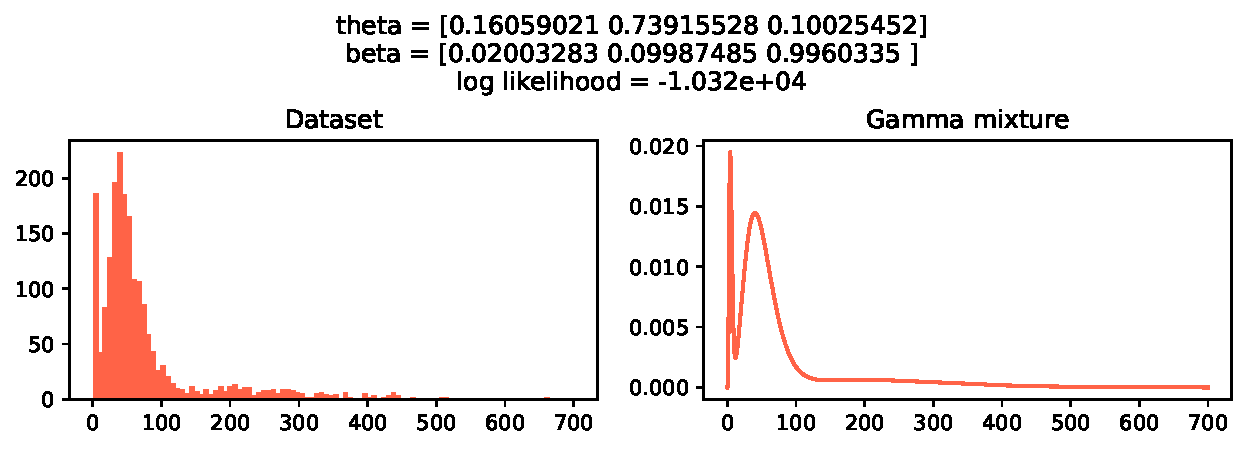
\includegraphics[width=\linewidth]{p1}

    Code:

    \begin{python}
def e_step(theta, betas):
    # expand x to have 3 copies of itself
    x_expand = np.column_stack((x,x,x))
    num = gamma.pdf(x_expand, a=alpha, scale = 1/betas) * theta
    q = num / np.reshape(np.sum(num, axis=1), (x.shape[0], 1))
    return q

def m_step(q):
    # theta_hat_k = sum_n{q_nk} / N
    theta_hat = np.sum(q, axis=0) / x.shape[0]  #kx1 vector
    
    # beta_hat_k = alpha * sum_n{q_nk} / sum_n{q_nk * x_k}
    # to calculate denom, expand x (Nx1) to 3 copies of self (Nx3) to multiply with q
    x_expand = np.column_stack((x,x,x))
    denom = np.sum(q * x_expand, axis=0)
    beta_hats = alpha * np.sum(q, axis=0) / denom
    
    return theta_hat, beta_hats

def log_px(x, theta, betas):
    log{sum_k{gamma(alpha,beta_k) * theta_k}}
    p = np.zeros(x.shape[0]) 
    for n in range(0, x.shape[0]):
        num = gamma.pdf(x[n], a=alpha, scale = 1/betas) * theta
        p[n] = np.log(np.sum(num)) 
    return p

def run_em(theta, betas, iterations=1000):
    for i in range(0, iterations):
        q = e_step(theta, betas)
        theta, betas = m_step(q)
    return theta, betas
    \end{python}
\end{enumerate}


\newpage

\begin{problem}[PCA, 15 pts]

% FDV: Here are the notes from last year.  I've already edited to make clear we want L2.  As noted below, we should also provide the baseline/reference to the pset 4 solutions in case they computed that wrong somehow.  
% 
% # problem 2 clarifications
% *NB: There was a lot of confusion about this problem, and we ended up accepting any form of comparison to PCA. Next year should clarify which norm students should use more explicitly (and maybe provide a baseline for students if the computation of the reconstruction error is different from what students calculated on pset4.)*
% 
% For Problem 2.3 (computing PCA reconstruction error), we will accept both the L1 and L2 norm and both summing over the errors for individual images and taking the mean of the errors (as long as you compute the error for K-Means the same way as you compute it for PCA). Apologies for the ambiguity in this question! 

  
For this problem you will implement PCA from scratch on the first 6000 images of the MNIST dataset. Your job is to apply PCA on MNIST and discuss what kind of structure is found. Implement your solution in \texttt{p2.ipynb} and attach the final plots below.

{\bfseries You will recieve no points for using third-party PCA implementations (i.e. {\normalfont \texttt{scikit-learn}}).}

{\bfseries You will recieve no points for code not included below.}
\begin{enumerate}

\item Compute the PCA. Plot the eigenvalues corresponding to the most
  significant 500 components in order from most significant to
  least. Make another plot that describes the cumulative proportion of
  variance explained by the first $k$ most significant components for
  values of $k$ from 1 through 500.  How much variance is explained by
  the first 500 components?  Describe how the cumulative proportion of
  variance explained changes with $k$.  Include this plot below.

\item Plot the mean image of the dataset and plot an image
  corresponding to each of the first 10 principle components.  How do
  the principle component images compare to the cluster centers from
  K-means? Discuss any similarities and differences.  Include these
  two plots below.

  \textit{Reminder: Center the data before performing PCA}

\item Compute the reconstruction error on the data set using the mean
  image of the dataset.  Then compute the reconstruction error using
  the first 10 principal components.  How do these errors compare to
  the final objective loss achieved by using K-means on the dataset?
  Discuss any similarities and differences.

  For consistency in grading, define the reconstruction error as the squared L2
  norm averaged over all data points.

\item Suppose you took the original matrix of principle components
  that you found $U$ and multiplied it by some rotation matrix $R$.
  Would that change the quality of the reconstruction error in the
  last problem?  The interpretation of the components?  Why or why
  not?
  
\end{enumerate}


\end{problem}

\newpage
\subsection*{Solution}
Plots:

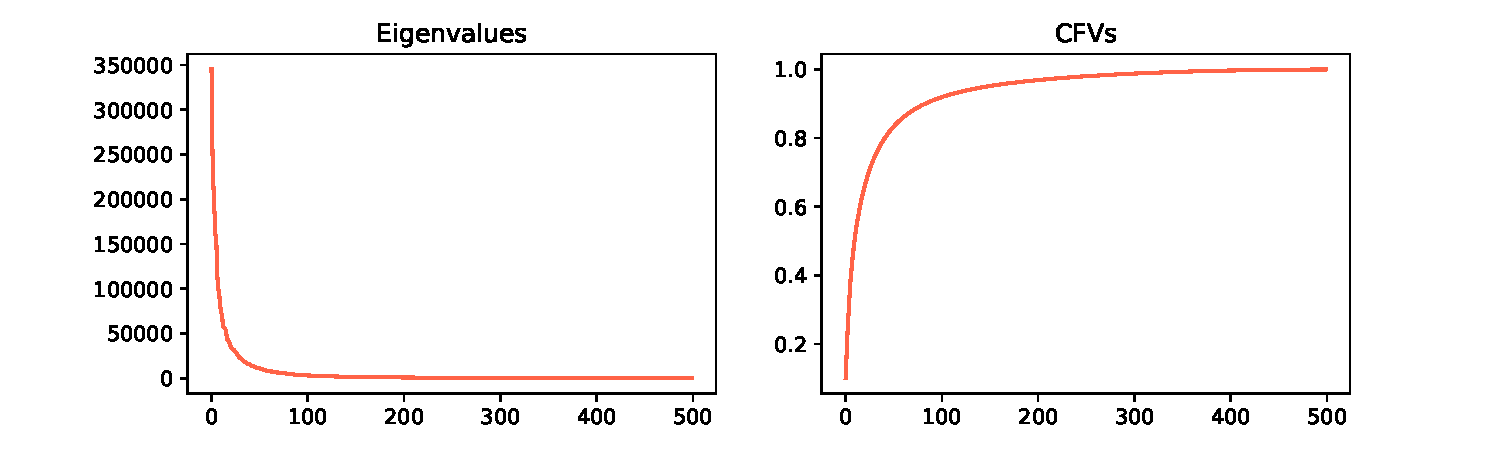
\includegraphics[width=\linewidth]{p2_cfvs}

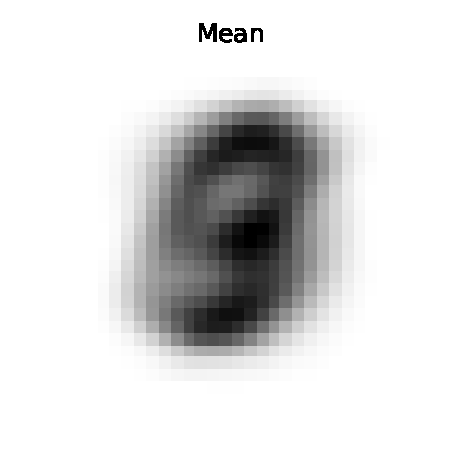
\includegraphics[width=0.25\linewidth]{p2_mean}
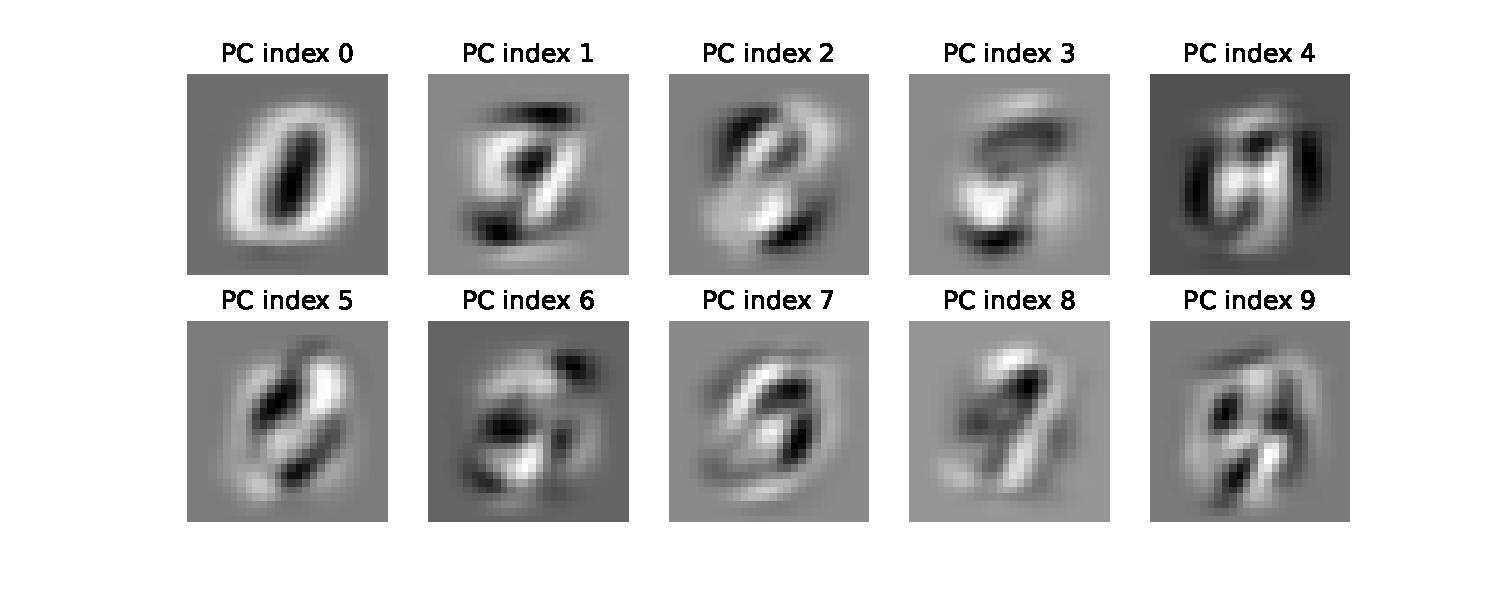
\includegraphics[width=0.75\linewidth]{p2_pcomps}

Code:

\begin{python}
def pca(x, n_comps=500):
    # make x mean-centered - center the columns before doing PCA
    centered_x = np.copy(x).astype(np.float64)
    for i in range(0, x.shape[1]):
        centered_x[:,i] = centered_x[:,i] - np.mean(x[:,i])
    
    U, Z, VT = np.linalg.svd(centered_x)
    
    # eigenvalues \lambda_i = z_i^2 / N
    top_eigvals = np.power(Z,2) / x.shape[0]
    
    # corresponding eigenvectors are rows of cols of V, ie rows of VT
    top_pcomps = VT   # principal components 
    
    
    # return the entire dataset
    return top_eigvals[0:n_comps], top_pcomps[0:n_comps, :]

def calc_cfvs(eigvals):
    cum_frac_vars = np.zeros(eigvals.shape[0])
    denom = np.sum(eigvals)
    for i in range(1,eigvals.shape[0]+1):
        cum_frac_vars[i-1] = np.sum(eigvals[0:i]) / denom
    return cum_frac_vars

def calc_errs(x, pcomps):
    mean_im = np.reshape(np.mean(x, axis=0), (1,784)) # 784x1 array
    err_mean = np.mean(np.linalg.norm(x - mean_im, axis=1)**2) 
    # mean_proj = (x @ mean_im) @ mean_im.T   # (x @ mean_im) is 6000x1 s.t. mean_proj is 6000x784
    # err_mean = np.mean(np.linalg.norm(x - mean_proj, axis=1)**2)         
    
    # reconstruction loss ||xn − (x · w)w||2 given w is vector which we project data onto
    # we are told to choose only first 10 principal components
    pcomp = pcomps[0:10, :].T  # 784x10 array
    pcomp_proj = (x @ pcomp) @ pcomp.T   # (x @ mean_pcomp) is 6000x10 s.t. pcomp_proj is 6000x784
    err_pcomp = np.mean(np.linalg.norm(x - pcomp_proj, axis=1)**2)
    
    return err_mean, err_pcomp
\end{python}

\begin{enumerate}
  \item As we see on the cummulative proportion of variance plot, the cummulative proportion of variance increases as k increases. When considering only the 500 most significant principal components, the first few most signifcant components cover the most amount of variance, the first 100 most significant components cover around 90\% of the variance, and all 500 components of course cover 100\% of the variance covered (when only considering these 500 components). \\
  Meanwhile, when considering all 784 principal components, the first 500 most significant principal components cover 99.93983\% of the total variance.
  
  \item \\
  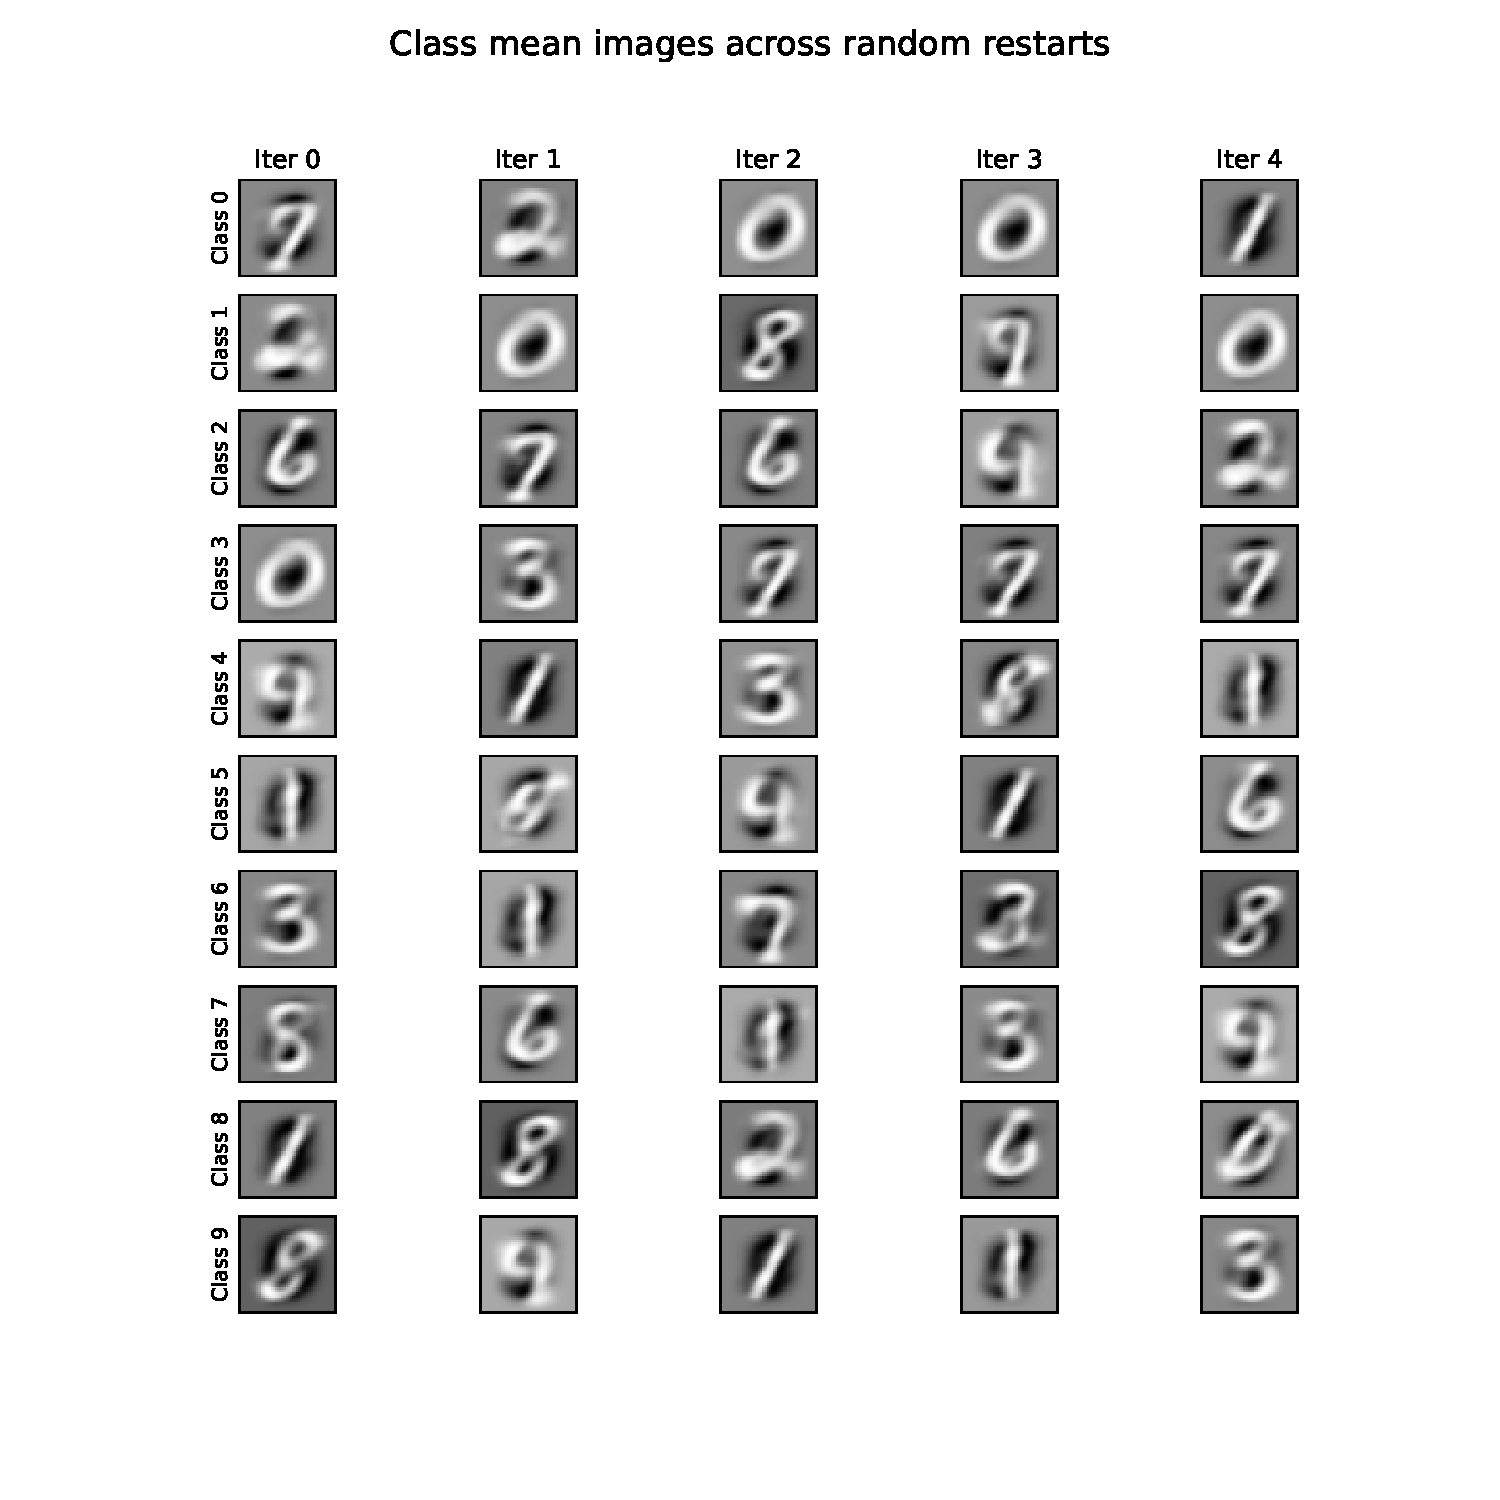
\includegraphics[width=0.75\linewidth]{HW5/k_means.pdf} \\
    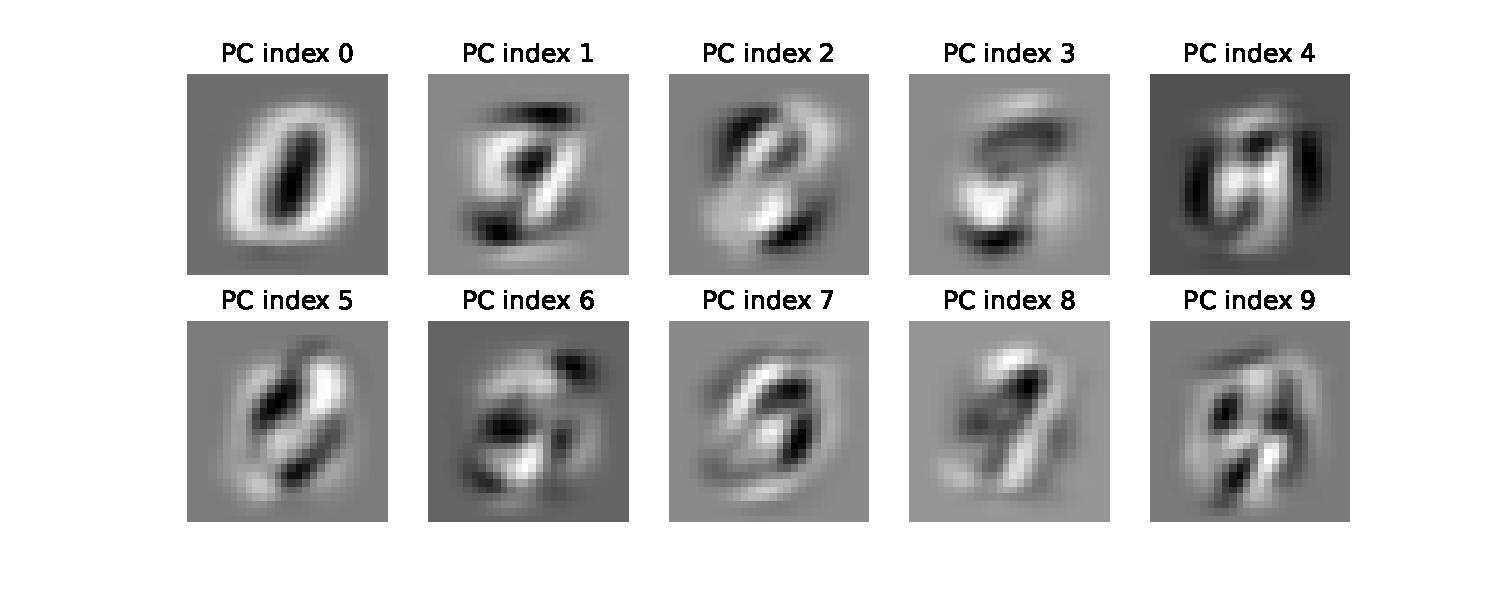
\includegraphics[width=0.75\linewidth]{p2_pcomps} \\

  We see that the top ten principal components from PCA are more blurry and less resemblant of any digits as compared to the cluster centers from K-means (which was run on the same mean-centered data as PCA). This makes sense, since the principal images which correspond to the highest variance axes of data don't necessarily correspond to digits, whereas clusters of similar-appearing images which were derived in K-means are more likely to appear as digits. \\
  We also see that digits such as 0 and 9 are seen in PCA and K-means, indicating that these are digits which have distinctly high variance relative to the dataset (as seen in PCA) and thus are able to (somewhat) precisely cluster together other digits which appear as 0 or 9 respectively (as seen in K-Means).

  \item
  The reconstruction error on the data set using the mean image of the dataset is $3.44 * 10^6$. \\
  The reconstruction error on the data set using the first 10 principal components is $1.92*10^6$. \\
  The final objective loss achieved by using K-means on the dataset (mean residual sum of squares) is $2.5*10^6$. \\
  We see that the reconstruction error using the mean image is the highest, which makes sense since the mean image is the least specific to any image in the dataset. Meanwhile, the reconstruction error for the first 10 principal components and K-Means are relatively very close, which makes sense since more images which match the data more closely are considered when reconstructing the error. PCA error is slightly lower than the K-Means error -- this makes sense since the PCA reconstruction error is choosing a linear combination of input images to construct principal images which have maximal variance, whereas K-means is not choosing cluster centers which have maximal variance and is dependent on the randomly initialized $\mu_k$'s when forming the cluster centers we converge to. 
  
  \item 
  Since the reconstruction loss is calculated by projecting the data onto the principal axis, and then computing the difference between the projected data and the actual data, if we rotate our principal component, we are now projecting the data onto a different vector (that is no longer the direction of variance that was intended). Since we are projecting the data onto a new vector that is not our original principal axis, the difference between the projected data and actual data will now lead to a different reconstruction error. \\
  Our interpretation of the principal components would also change - a principal component which was originally a vector pointing in the direction of maximal variance will no longer point in the direction after rotation. 
\end{enumerate}

\newpage

\begin{problem}[Bayesian Networks, 10 pts]

% FDV: I think we can keep this problem as-is, and just clarfiy based
% on notes from last year.
% # problem 3 clarifications
% The phrasing of Q3 is slightly off because it implies that you need to explain why each path is not blocked in the case that two nodes are not independent. It is sufficient to provide a single unblocked path. Better phrasing is (emphasis added) "Use the concept of d-separation to answer the questions and show your work (i.e., state what the blocking path(s) is/are and which node blocks the path; or explain why there exists a path that is not blocked)." 
% 
% Some helpful resources for d-separation:  The 2020 Section 8 notes, Bishop p. 372 - 379, Section 8.2 of the CS 181 textbook
% 
% Problem 3: Make it clear (put the instructions in one place) that we require explanations for both "yes" and "no" answers

  
  \noindent In this problem we explore the conditional independence
  properties of a Bayesian Network.  Consider the following Bayesian
  network representing a fictitious person's activities. Each random
  variable is binary (true/false).

\begin{center}
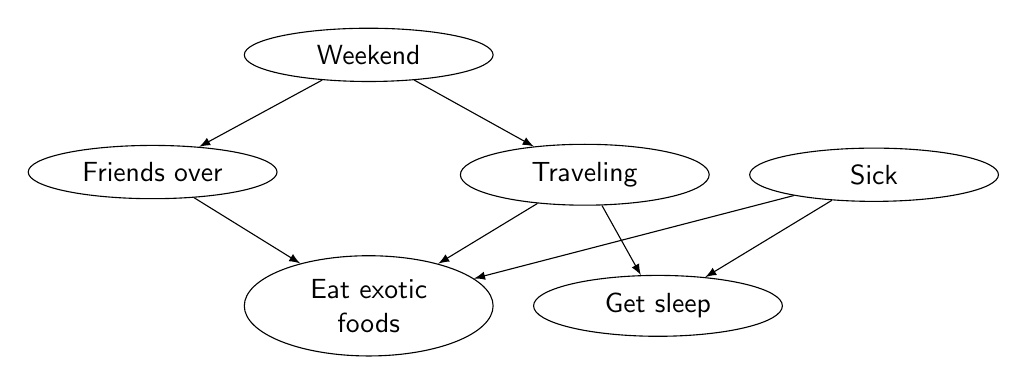
\begin{tikzpicture}[
  node distance=1cm and .5cm,
  bn/.style={draw,ellipse,text width=2cm,align=center}
    ]
    \node[bn] (w) {\attr{Weekend}};
    \node[bn,below right=of w] (t) {\attr{Traveling}};
    \node[bn,right=of t] (s) {\attr{Sick}};
    \node[bn,below left=of w] (f) {\attr{Friends over}};
    \node[bn,below right=of f] (eef) {\attr{Eat exotic foods}};
    \node[bn,right=of eef] (gs) {\attr{Get sleep}};
    \path (w) edge[-latex] (t)
    (w) edge[-latex] (f)
    (f) edge[-latex] (eef)
    (t) edge[-latex] (eef)
    (t) edge[-latex] (gs)
    (s) edge[-latex] (gs)
    (s) edge[-latex] (eef);
    \end{tikzpicture}
\end{center}

The random variables are:

\begin{itemize}
\item \attr{Weekend}: Is it the weekend?
\item \attr{Friends over}: Does the person have friends over?
\item \attr{Traveling}: Is the person traveling?
\item \attr{Sick}: Is the person sick?
\item \attr{Eat exotic foods}: Is the person eating exotic foods?
\item \attr{Get Sleep}: Is the person getting sleep?
\end{itemize}

\medskip

For the following questions, $A \perp B$ means that events A and B are
independent and $A \perp B | C$ means that events A and B are independent
conditioned on C.

\textbf{Use the concept of d-separation} to answer the
questions and show your work (i.e., state what the blocking path(s) is/are and what nodes block the path; or explain why each path is not blocked).

\textit{Example Question:} Is $\attr{Friends over} \perp \attr{Traveling}$? If NO, give intuition for why.

\textit{Example Answer:} NO. The path from Friends over -- Weekend -- Traveling is not blocked following the d-separation rules as we do not observe Weekend. Thus, the two are not independent. 

\textbf{Actual Questions:}

\begin{enumerate}
\item Is $\attr{Weekend} \perp \attr{Get Sleep}$?
  If NO, give intuition for why.

\item Is $\attr{Sick} \perp \attr{Weekend}$?
  If NO, give intuition for why.


\item Is $\attr{Sick} \perp \attr{Friends over}\given \attr{Eat exotic
  foods}$? If NO, give intuition for why.


\item Is $\attr{Friends over} \perp \attr{Get Sleep}$? If NO, give
  intuition for why.

\item Is $\attr{Friends over} \perp \attr{Get Sleep} \given
  \attr{Traveling}$? If NO, give intuition for why.

\item Suppose the person stops traveling in ways that affect their
  sleep patterns.  Travel still
  affects whether they eat exotic foods.  Draw the modified network. (Feel free to reference the handout file for the commands for displaying the new network in \LaTeX).

\item For this modified network, is $\attr{Friends over} \perp
  \attr{Get Sleep}$? If NO, give an intuition why.  If YES,
  describe what observations (if any) would cause them to no longer be
  independent.

\end{enumerate}
\end{problem}

\newpage
\section*{Solution}
\begin{enumerate}
  \item No. Since Travelling is not observed, by d-separation rules the path from Weekend to Travelling to Get Sleep is not blocked. Thus, Weekend and Get Sleep are not independent.
  
  \item Yes. Since Get Sleep is not observed and Eat Exotic Foods is not observed, the path from Sick -- Get Sleep  -- Travelling is blocked, Sick -- Eat Exotic Foods -- Travelling is blocked, and and Sick -- Eat Exotic Foods -- Friends Over is blocked. Since these three paths are all the undirected paths which can be taken from Sick to Weekend, every path is blocked, and by d-separation rules, Sick and Weekend are independent. 
  
  \item  No. Since we observe Eat Exotic Foods, the path Sick -- Eat Exotic Foods -- Friends Over is not blocked. Thus, by d-separation rules, Sick and Friends are not independent given Eat Exotic Foods.
  
  \item No. Since Weekend is not observed, the path Friends Over -- Weekend -- Travelling is unblocked. Since Travelling is not observed, the path Weekend -- Travelling -- Get Sleep is unblocked. Therefore, the path Friends Over -- Weekend -- Travelling -- Get Sleep is unblocked, and by d-separation rules, Friends Over and Get Sleep are not independent. 
  
  \item Yes. (only need to explain why if answer is No).
  
  
  \item  \\
  \begin{center}
    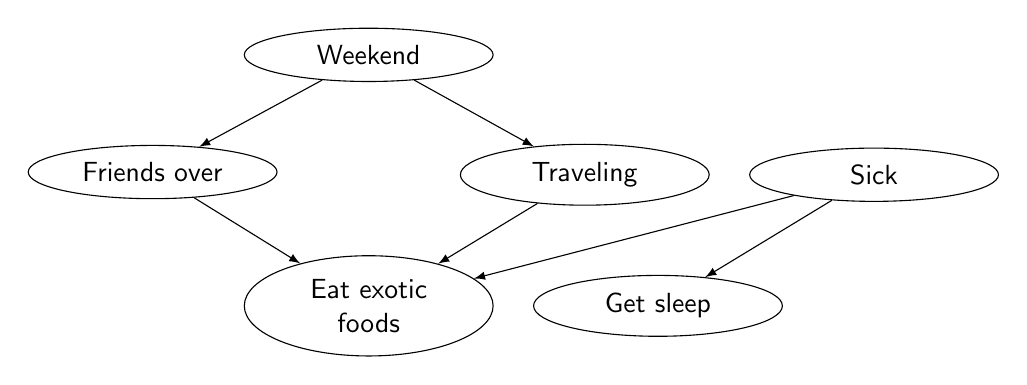
\begin{tikzpicture}[
      node distance=1cm and .5cm,
      bn/.style={draw,ellipse,text width=2cm,align=center}
        ]
        \node[bn] (w) {\attr{Weekend}};
        \node[bn,below right=of w] (t) {\attr{Traveling}};
        \node[bn,right=of t] (s) {\attr{Sick}};
        \node[bn,below left=of w] (f) {\attr{Friends over}};
        \node[bn,below right=of f] (eef) {\attr{Eat exotic foods}};
        \node[bn,right=of eef] (gs) {\attr{Get sleep}};
        \path (w) edge[-latex] (t)
        (w) edge[-latex] (f)
        (f) edge[-latex] (eef)
        (t) edge[-latex] (eef)
        (s) edge[-latex] (gs)
        (s) edge[-latex] (eef);
        \end{tikzpicture}
    \end{center}
  \item Yes. Friends Over and Get Sleep are Independent. Observe that in our new model, the only two undirected paths from Friends Over to Get Sleep are 
  \begin{enumerate}
      \item Friends Over -- Weekend -- Travelling -- Eat Exotic Foods -- Sick -- Get Sleep   
      \item Friends Over -- Eat Exotic Foods -- Sick -- Get Sleep
  \end{enumerate}
  In order for Friends Over and Get Sleep to no longer be independent, then we need to unblock at least one of these two paths at some node. Observing Eat Exotic Foods unblocks (a) and (b). (This is the only observation that leads to unblocking, as changing any other observation from what it currently is will lead to additional blockage of the undirected path(s) instead of unblockage, which could not help us in making Friends Over and Get Sleep dependent).
  
\end{enumerate}

\newpage
%%%%%%%%%%%%%%%%%%%%%%%%%%%%%%%%%%%%%%%%%%%%%
% Name and Calibration
%%%%%%%%%%%%%%%%%%%%%%%%%%%%%%%%%%%%%%%%%%%%%
\subsection*{Name}
Arnav Srivastava
\subsection*{Collaborators and Resources}
Whom did you work with, and did you use any resources beyond cs181-textbook and your notes? \\
Chinmay Deshpande. No resources were used beyond the textbook.

\subsection*{Calibration}
Approximately how long did this homework take you to complete (in hours)? \\
20

\end{document}
